\chapter{Introduction to Complex Numbers}

The extension from the real numbers to the complex numbers has far-reaching affects.  In this chapter, we give a brief introduction to complex numbers and then show how they interact with almost every topic in the course!

\section{Complex Numbers} 
The complex numbers arise out of the fact that the simple little equation $x^2+1=0$ has no solution over the reals.  Thus, we create \complex{the number $i$} to represent a root of that polynomial.  That is, $i^2+1=0$.  
\begin{definition}{Complex Numbers}  The set of \emph{complex numbers} is the set of all numbers that can be written in the form $a+bi$ for real numbers $a$ and $b$.
\end{definition}

We perform arithmetic in the complex numbers using the usual rules of arithmetic and algebra along with the extra identity $i^2=-1$.

\begin{exercise}{Containment of the Reals \Coffeecup}
\begin{itemize}
\item Is 3 a complex number?  Can you write 3 in the form $a+bi$ for real numbers $a$ and $b$?
\vspace*{.5in}
\item Does the set of complex numbers contain all real numbers?
\vspace*{.5in}
\end{itemize}
\end{exercise}

We can visualize complex numbers in the complex plane, where $a$ (the \emph{real part}) is the horizontal component and $b$ (the \emph{imaginary part}) is the vertical. 

\begin{center} 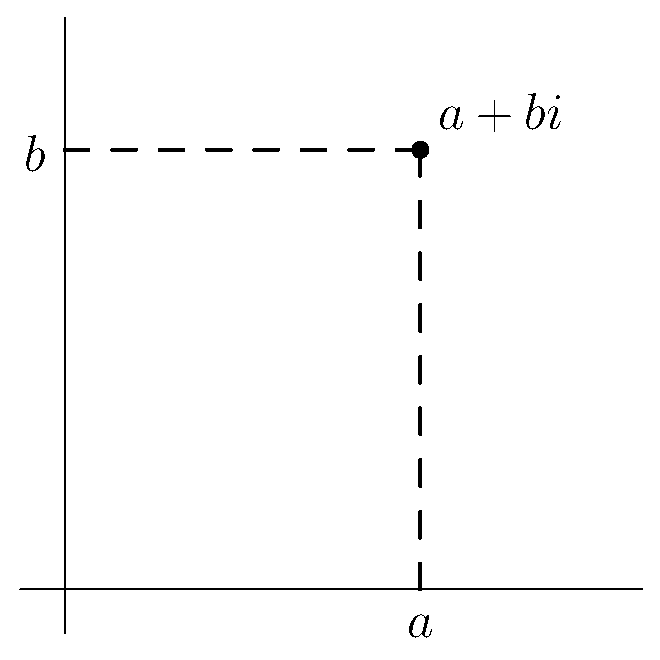
\includegraphics[width=200pt]{ChapterComplex/Figures/complexcart.eps}
\end{center}

\section{Euler's Identity and Consequences}

Look again at the power series for the exponential function, sine, and cosine: 
\begin{align*}
e^x&=1+x+\frac{1}{2!}x^2+\frac{1}{3!}x^3+\frac{1}{4!}x^4+\frac{1}{5!}x^5+\frac{1}{6!}x^6+\frac{1}{7!}x^7+\cdots\\
\cos(x)&=1-\frac{1}{2!}x^2+\frac{1}{4!}x^4-\frac{1}{6!}x^6+\cdots \\
\sin(x)&=x-\frac{1}{3!}x^3+\frac{1}{5!}x^5-\frac{1}{7!}x^7+\cdots \\
\end{align*}

You have to wonder if there is some way to add together sine and cosine to get the exponential function!  Sure the signs are off, but otherwise things seem so right.  Sine has all the odd factorial denominators, cosine has all the even factorial denominators, and the exponential function has all of them!  It turns out that $i$ is exactly the constant we need to fix those minus signs!

\begin{exercise}{\euleridentity{Proof of} Euler's Identity \Coffeecup \Coffeecup}
\begin{itemize}
\item Write out a power series for $e^{i\theta}$. \vspace*{2in}
\item Write out a power series for $\cos(\theta)+i\sin(\theta)$.\vspace*{2in}
\item Verify the two are equal!
\vspace*{1in}
\end{itemize}
\end{exercise}

The fact that there is any relationship whatsoever between sine, cosine, and $e$ is very surprising when you think of how differently those quantities are defined!  We again state this incredible theorem, \complex{Euler's Identity}! 

\begin{theorem}{Euler's Identity}
For any real number $\theta$, $$e^{i\theta}=\cos(\theta)+i\sin(\theta). $$
\end{theorem}

If we multiply both sides by a real number $r$, we then obtain $$ re^\theta=r\cos(\theta)+ir\sin(\theta).$$
We notice that the horizontal component, $r\cos(\theta)$, is in fact the conversion for $x$ into polar coordinates.  Likewise, $r\sin(\theta)$ is the conversion for $y$ into polar coordinates.  This means that the \polar{complex number} $re^{i\theta}$ is in fact the point located at angle $\theta $ and radius $r$ in the complex plane.  
\begin{center}	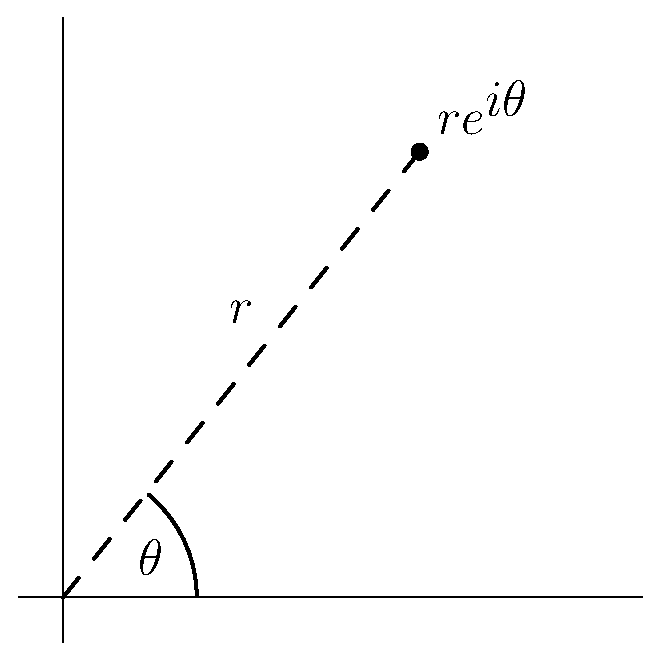
\includegraphics[width=200pt]{ChapterComplex/Figures/polarcart.eps}
\end{center}

\subsection{Complex Roots}
 
One interesting fact about the complex numbers is that the number of $n^{th}$ roots of \emph{every} real number is exactly $n$.  So every number has two square roots, three cubed roots, and so on.  We use $re^{i\theta}$ form to find these \complex{complex roots}.

\begin{example}{The Cubed Roots of Two} To find all cubed roots of two, we solve the equation $$z^3=2. $$
We begin by putting both $z$ and $2$ in complex polar form.  We write $z=re^{i\theta}$ and $2=2e^{i0}$.  We plug these into the equation, expand the powers. \begin{align*}
z^3&=2 \\
\left(re^{i\theta}\right)^3&=2e^{i0} \\
r^3e^{i3\theta}&=2e^{i0} \\
\end{align*}
 
 We now equate the radius and the angles as two separate equations.
 
 \begin{itemize}
 \item {\bf Radius:} Since $r$ is a real number, we obtain $r^3=2$, which implies $r=\sqrt[3]{2}$.
 \item {\bf Angle:} The angles need to be equivalent but not necessarily equal.  If they differ by a multiple of $2\pi$, that is fine!  Thus, we have $3\theta = 0 + 2\pi k$ for any integer $k$.  Dividing both sides by 3, we have $$\theta=\frac{0 + 2\pi k}{3} =\ldots,\frac{-4\pi}{3},\frac{-2\pi}{3},0,\frac{2\pi}{3},\frac{4\pi}{3},\frac{6\pi}{3},\ldots. $$
However, if we use more values of $\theta$ beyond just $0,\frac{2\pi}{3},\frac{4\pi}{3}$, the solutions will repeat since cosine and sine have period $2\pi$. Thus, we use just those three angles.
 \end{itemize}
 Putting together our $r$ and $\theta$ values, we have the following three roots: $$z=\sqrt[3]{2}e^{i0},\sqrt[3]{2}e^{i\frac{2\pi}{3}},\sqrt[3]{2}e^{i\frac{4\pi}{3}} .$$

Thus, we have our \euleridentity{roots} in complex polar form.  We use Euler's Identity to turn these back into complex cartesian form as follows:
$$z=\sqrt[3]{2}\cos(0)+i\sqrt[3]{2}\sin(0),\sqrt[3]{2}\cos(\frac{2\pi}{3})+i\sqrt[3]{2}\sin(\frac{2\pi}{3}),\sqrt[3]{2}\cos(\frac{4\pi}{3})+i\sqrt[3]{2}\sin(\frac{4\pi}{3}).$$
At last, we use the unit circle to evaluate these and plot in the complex plane. 
$$z=\sqrt[3]{2},-\frac{\sqrt[3]{2}}{2}+i\frac{\sqrt[3]{2}\sqrt{3}}{2},-\frac{\sqrt[3]{2}}{2}-i\frac{\sqrt[3]{2}\sqrt{3}}{2}$$

\begin{center}
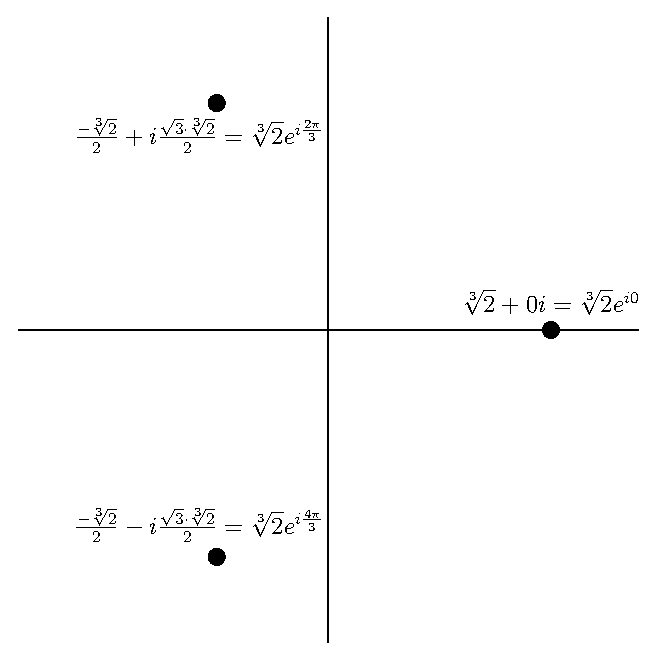
\includegraphics[width=200pt]{ChapterComplex/Figures/cuberoot2.eps}
\end{center}

\end{example}

\begin{exercise}{Checking Once Again \Coffeecup \Coffeecup}
Cube each of the answers from the previous problem.  Verify in each case you get 2!
\vspace*{3in}
\end{exercise}

It turns out to be of particular importance to find roots of 1.  Define the \emph{$n^{th}$ roots of unity } to be the solutions to the equation  

$$ z^n =1. $$

Lets play around and see if we can find some neat properties!
\begin{exercise}{Roots of Unity \Coffeecup \Coffeecup \Coffeecup \Coffeecup}
\begin{itemize}

\item Find all square roots of unity.  Write your answers in both cartesian and polar complex form, and plot them in the complex plane.  (the case where $n=2$)

\vspace*{2in}

\item Find all third roots of unity.
\vspace*{2in}

\item Find all fourth roots of unity.

\vspace*{1.5in}

\item Find all fifth roots of unity.

\vspace*{1.5in}

\item Find all sixth roots of unity.

\vspace*{1.5in}

\item Fill out the following table:
\begin{center}
\begin{tabular}{|c|c|c|}
 \hline
  $n$ & $\Sigma_n$ & $\Pi_n$ \\
  \hline \hline  
  2 & \hspace{.2in} & \hspace{.2in} \\   \hline
  3 & \hspace{.2in} & \hspace{.2in} \\   \hline
  4 & \hspace{.2in} & \hspace{.2in} \\   \hline
  5 & \hspace{.2in} & \hspace{.2in} \\   \hline
  6 & \hspace{.2in} & \hspace{.2in} \\   \hline
  \hline
\end{tabular}
\end{center}

where $\Sigma_n$ represents the sum of all $n^{th}$ roots of unity and $\Pi_n$ represents the product of all $n^{th}$ roots of unity.  ({\bf Hint:} It's easier to add in cartesian, and easier to multiply in polar.)

\item Based on your above data gathered, conjecture a formula for both $\Sigma_n$  and $\Pi_n$.  Prove your conjecture is correct.  ({\bf Hint:} Consider the roots of the polynomial $z^n-1$ and how that polynomial would factor based on those roots.  Then consider the degree zero and degree $n-1$ coefficients.)

\vspace*{2in}

\end{itemize}
\end{exercise}

Using the same techniques we can answer the following question, ``what is the square root of $i$?''  Keep in mind there are technically two square roots of $i$, the two solutions to the equation $z^2=i$.

\begin{exercise}{Square Roots of $i$ \Coffeecup \Coffeecup}
\begin{itemize}

\item Find the square roots of $i$.  Write your answers in complex cartesian form.

\vspace*{2in}

\item Square your answers back out (in complex cartesian form) and verify that you do in fact get $i$ when you square them.

\vspace*{2in}

\end{itemize}
\end{exercise}

\begin{exercise}{Cubed Roots of $i$ \Coffeecup \Coffeecup \Coffeecup}
\begin{itemize}

\item Find all cubed roots of $i$.  That is, find all complex numbers $z$ such that $z^3=i$.  Write your answers in $a+bi$ form. 

\vspace*{2in}

\item Take the cube of each of your roots to verify that you do in fact get $i$ as the third power.

\vspace*{2in}

\end{itemize}
\end{exercise}

\subsection{\trigidentities{Proving Trig Identities}}

Remember how there are 47,000 useful but impossible to remember \complex{trigonometric identities}?  No?  Well, that shows how hard they are to remember.  Believe it or not, most of them can be constructed very quickly and easily from \doubleangle{Euler's Identity}!  

\begin{example}{The Sine and Cosine Double-Angle Identities}
To construct the sine and cosine double-angle formulas, we can manipulate the expression $e^{2\theta}$.  We proceed with the following chain of equality:
\begin{align*}
\cos(2\theta)+i\sin(2\theta)&=e^{i\cdot 2\theta} \\
&=\left(e^{i\theta} \right)^2 \\
&=\left(\cos(\theta)+i\sin(\theta) \right)^2\\ 
&=\cos^2(\theta)+2\cos(\theta)i\sin(\theta)+i^2\sin^2(\theta)  \\
&=\left(\cos^2(\theta)-\sin^2(\theta)\right)+i\left(2\sin(\theta)\cos(\theta) \right). 
\end{align*}
We now equate real parts to obtain the cosine double-angle identity $$\cos(2\theta)=\cos^2(\theta)-\sin^2(\theta). $$

Similarly, we equate imaginary parts to obtain the sine double-angle identity
$$\sin(2\theta)=2\sin(\theta)\cos(\theta). $$
\end{example}

\begin{exercise}{Annotate! \Coffeecup}
Write a short justification alongside each line of computation above.
\end{exercise}

\begin{exercise}{Angle-Sum Identities \Coffeecup \Coffeecup}
\begin{itemize}
\item Expand the expression $e^{i(A+B)}$ into real and imaginary parts using Euler's Identity.
\vspace*{2in}
\item Expand the expression $e^{iA}e^{iB}$ into real and imaginary parts using Euler's Identity twice, once per factor.  Multiply out the resulting terms into an expression of the format $$f(A,B)+ig(A,B)$$ where $f$ is the function corresponding the real part of that expression, and $g$ corresponds to the imaginary part.
\vspace*{2in}
\item Equate real and imaginary parts to produce the angle sum identities for $\cos$ and $\sin$, respectively!  ({\bf Hint:} We're using the fact that two complex numbers $a+bi$ and $c+di$ are equal if and only if $a=c$ and $b=d$.)
\vspace*{2in}
\end{itemize}
\end{exercise}

\subsection{Natural Logarithm of a Complex Number}\label{ComplexLogs}

\begin{wrapfigure}{r}{0.3\textwidth}
    	\centering
		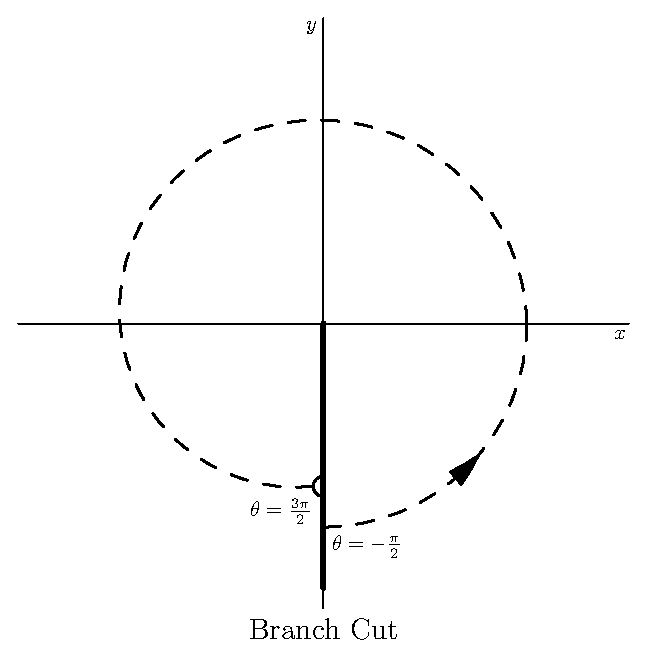
\includegraphics[width=0.3\textwidth]{ChapterComplex/Figures/BranchCut}
\end{wrapfigure}

We now show how to compute the \complex{natural logarithm} of a complex number.  As usual, polar form will be critical.

\begin{itemize}
\item Given a complex number $z$, we first write $z$ in polar form $z=re^{i\theta}$, where $r$ is a positive real number and $\theta \in [-\pi/2,3\pi/2)$.  This choice of interval for $\theta$ is often called a \emph{branch cut} and is essentially a domain restriction for the exponential function (since it fails to be one-to-one over the complex numbers).

\item Split apart using the property of logarithms and cancel the log with the exponential as follows: $$ \ln(z)=\ln\left( re^{i\theta}\right)=\ln(r)+\ln\left( e^{i\theta} \right) =\ln(r)+i\theta.$$
\end{itemize}

\vspace*{.1in}

\begin{example}{Natural Log of $i$}\label{LogOfi}
Here we compute the mysterious quantity $\ln(i)$.  We begin by rewriting $i$ as $$i=1\cdot e^{i\pi/2}. $$  Notice that we chose the angle $\theta=\pi/2$ to be within the branch cut specified above.  From here, we split using log properties as follows:  \begin{align*}
\ln(i)&=\ln\left(1\cdot e^{i\pi/2} \right)\\
&=\ln\left(1  \right) + \ln\left(e^{i\pi/2}  \right)\\
&=0 + i\frac{\pi}{2}. 
\end{align*}
Thus, $\ln(i)=\frac{\pi}{2}i.$
\end{example}

Note that in principle there is no reason we had to pick our angle $\theta$ in that particular interval.  One can construct a perfectly well-defined logarithm from choosing a different domain for $\theta$.  This is similar to the construction of the inverse trig functions, where one must restrict the domain in some manner, so we tend to just choose a default interval to restrict to and stick with it.

\begin{exercise}{Complex Logarithms \Coffeecup \Coffeecup}

Try the above method to compute each of the following logarithms.  Write each in the standard complex cartesian form $a+bi$.

\begin{itemize}
\item $\ln(2)$
\vspace{.5in}
\item $\ln(-2)$
\vspace{.5in}
\item $\ln(1+i)$
\vspace{.5in}
\item $\ln(3-4i)$
\vspace{.5in}
\end{itemize}
\AnswerKeyEntry{\textbullet $\ln(2)=\ln(2)+0i$
\textbullet $\ln(-2)=\ln(2)+\pi i$ \textbullet $\ln(1+i)=\ln\left(\sqrt{2}\right)+i\frac{\pi}{4}$ 
\textbullet $\ln(3-4i)=\ln(5)+i\arctan\left(-\frac{3}{4}\right)$}
\end{exercise}

\subsection{Complex Exponentials}

Recall our trick for dealing with strange bases: $${w_1}^{w_2}=e^{\mathtt{ln}{\left( {w_1}^{w_2} \right) }}=e^{w_2\mathtt{ln}{\left( w_1 \right)}}.$$
This provides the advantage of moving us back to the familiar base $e$ from the unfamiliar base $w_1$.  This will make a complex \complex{exponential} base manageable!

\begin{example}{Computation of Hammurabi}
Here we perform two exponentials; we have an $i$ to an $i$, and a 2 to the $2^{th}$.  Using the above trick and the value of $\ln(i)$ computed in Example \ref{ComplexLogs}.\ref{LogOfi}, we find

\begin{align*}
i^i2^2&=4i^i\\
&=4e^{\ln\left(i^i\right)}\\
&=4e^{i\ln\left(i\right)}\\
&=4e^{i\frac{\pi}{2}i}\\
&=4e^{-\frac{\pi}{2}}.
\end{align*}
Notice there was no need to decompose further using Euler's Identity here; the end result of $i$ raised to the $i$ power is in fact a real number!
\end{example}

\begin{exercise}{Complex Exponentials \Coffeecup \Coffeecup}
\begin{itemize}
\item Use the above trick to compute $(1+i)^i$.
\vspace*{1in}
\item Use the above trick to compute $i^{1+i}$.
\vspace*{1in}
\item Use the above trick to compute $(1+i)^{1+i}$.
\vspace*{1in}
\end{itemize}
\AnswerKeyEntry{The number $(1+i)^{1+i}$ can be written in complex cartesian form as $$\left(e^{\ln\left(\sqrt{2}\right)-\frac{\pi}{4}}\cos\left(\ln\left(\sqrt{2}\right)+\frac{\pi}{4} \right)\right)+i\left(e^{\ln\left(\sqrt{2}\right)-\frac{\pi}{4}}\sin\left(\ln\left(\sqrt{2}\right)+\frac{\pi}{4} \right)\right). $$}
\end{exercise}

\section{Partial Fractions via Complex Numbers}
If we are using \partialfractions{complex numbers}, there are no more irreducible quadratics!  This gives us an interesting alternate way to perform \complex{PFD}, since all polynomials will fully factor into linear factors.
\begin{exercise}{PFD over the Complex Numbers \Coffeecup \Coffeecup \Coffeecup}

\begin{itemize}
\item Find an antiderivative of $\frac{4-2 x^2}{x^3+4 x}$ via a partial fraction decomposition over the real numbers.
\vspace*{3in}

\item Find an antiderivative of $\frac{4-2 x^2}{x^3+4 x}$ via a partial fraction decomposition \antider{over the complex numbers}.

\vspace*{3in}

\item Verify your answers are compatible.

\vspace*{1in}

\end{itemize}
\AnswerKeyEntry{The PFD over the complex numbers is $$\frac{4-2x^2}{x^3+4x}=\frac{1}{x}-\frac{\frac{3}{2}}{x+2i}-\frac{\frac{3}{2}}{x-2i}. $$}
\end{exercise}

Since Euler's Identity relates the exponential function to trigonometric functions, it is plausible that there would be analagous relationships out there between logarithmic and inverse trigonometric functions over the complex numbers!  At a very crude level, one can think of just taking an inverse function of both sides of Euler's Identity.  It turns out that PFD over the complex numbers is the right tool to make this formal!

\begin{exercise}{Inverse Tangent and Natural Log}
Recall that by trigonometric substitution, we have $$\int \frac{1}{x^2+1}\dif x=\arctan(x)+C. $$  Compute the same antiderivative but using a PFD over the complex numbers.  In particular, carry out the following steps:
\begin{itemize}
\item Factor $x^2+1$ over the complex numbers.
\vspace*{.5in}
\item Find $A$ and $B$ in the decomposition $$\frac{1}{x^2+1}=\frac{A}{x+i}+\frac{B}{x-i}. $$
\vspace*{1in}
\item Find the antiderivative, simply integrating terms of the form $\frac{c_1}{x+c_2}$ as $c_1\ln\left(x+c_2\right)$ for complex constants $c_1$ and $c_2$, just as you would for real constants.
\vspace*{1in}
\item Conclude that $$\arctan(x) = \frac{1}{2i} \ln\left(\frac{x-i}{x+i}\right) + C$$ for some constant $C$.
\vspace*{1in}
\item Solve for $C$ by letting $x\to \infty$ on both sides to get a relationship between inverse tangent and the natural logarithm! (It is valid for positive $x$.)
\vspace*{1in}

\end{itemize}
\AnswerKeyEntry{In taking the limit, the logarithmic term will approach zero.  Thus $C=\pi/2$.}

\end{exercise}
